\documentclass[a4paper]{article}

\usepackage[english]{babel}
\usepackage[utf8]{inputenc}
\usepackage{indentfirst}
\usepackage{graphicx}
\usepackage{verbatim}
\usepackage{float}
\usepackage{url}
\usepackage[color]{vdmlisting}
\usepackage{longtable}
\usepackage[hidelinks]{hyperref}
\usepackage{fullpage}

\begin{document}

\setlength{\textwidth}{16cm}
\setlength{\textheight}{22cm}

\title{\Huge\textbf{Formal Modelling of a Petri Net in VDM++}\linebreak\textbf{}\linebreak\linebreak
\Large\textbf{Final Report}\linebreak\linebreak

\includegraphics[height=6cm, width=7cm]{feup.pdf}\linebreak \linebreak
\Large{Master in Informatics and Computing Engineering} \linebreak \linebreak
\Large{Formal Methods in Software Engineering}\linebreak
}

\author{\textbf{Group T03\_3:}\\ Duarte Nuno Pereira Duarte - ei11101 \\ Ruben Fernando Pinto Cordeiro - ei11097 \\\linebreak\linebreak \\
 \\ Faculdade de Engenharia da Universidade do Porto \\ Rua Roberto Frias, s\/n, 4200-465 Porto, Portugal \linebreak\linebreak\linebreak
\linebreak\linebreak\vspace{1cm}}
%\date{Junho de 2007}
\maketitle

\thispagestyle{empty}
\newpage
\tableofcontents

%************************************************************************************************
%************************************************************************************************

\newpage

\section {Summary}

The goal of this project is to model the structure and behaviour of a Petri net in VDM++.

A Petri net is mathematical modelling language for the description of distributed systems. It is typically represented by a graphical notation for stepwise processes that include choice, iteration and cocurrent execution.

In order to build the executable formal model, the model-oriented specification language from the \emph{Vienna Development Method} (VDM++) was used, as well as the Overture Tool\cite{Overture} for development.

\newpage

\section {System Description}
\label{sec:system_description}

Petri nets are a graphical and mathematical modeling tool applicable to many systems. As a graphical tool, Petri nets can be used as a visual-communication aid similar to flow charts, block diagrams and netweorks. In addition, tokens are used in these nets to simulate the dynamic and concurrent activities of systems.

\begin{figure}[h]
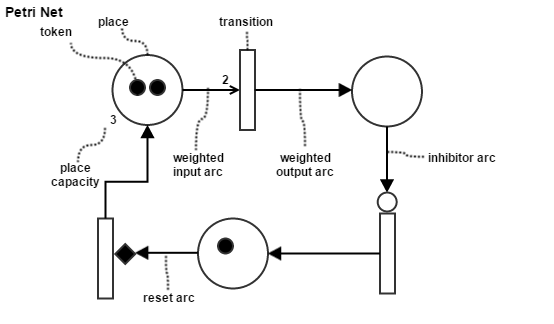
\includegraphics[width=17cm]{petrinet.png}
\caption{Petri net graphical structure}
\end{figure}

A Petri net is a directed bipartite graph, in which the nodes represent transitions (i.e. events that may occur, signified by bars) and places (i.e. conditions, signified by circles). The directed arcs describe which places are pre- and/or postconditions for which transitions (signified by arrows).

A Petri net can be described as a 5-tuple, $PN = (P, T, F, W, M_0)$, where: 

\begin{itemize}
	\item [P] = $\{p_1, p_2, ..., p_m\}$ is a finite set of places.
    \item [T] = $\{t_1, t_2, ..., t_n\}$ is a finite set of transitions.
    \item [F] $\subseteq (P \times T) \bigcup (T \times P)$ is a set of arcs.
    \item [W]: $F \rightarrow \{1, 2, 3, ...\}$ is a weight function.
    \item [$M_0$]: $P \rightarrow \{0, 1, 2, 3, ...\}$ is the initial marking.
\end{itemize}

Graphically, places in a Petri net may contain a discrete number of marks called tokens. Any distribution of tokens over the places will represent a configuration of the net called a marking. In an abstract sense relating to a Petri net diagram, a transition of a Petri net may fire if it is enabled, i.e. there are sufficient tokens in all of its input places; when the transition fires, it consumes the required input tokens, and creates tokens in its output places. A firing is atomic, i.e., a single non-interruptible step.

\subsection{Arc types and firing rules}

There are three types of arcs:

\begin{itemize}
	\item Weighted arcs.
    \item Inhibitor arcs.
    \item Reset arcs.
\end{itemize}

The state or marking in a Petri net is changed according to a firing rule for a transition t.

A reset arc does not impose a precondition on firing: the transition is always enabled and the place is emptied when the transition fires.

An inhibitor arc imposes the precondition that the transition may only fire when the place is empty.

If the arc is weighted, the following firing rule applies:

\begin{enumerate}
	\item A transition t is said to be enabled is each input place \textit{p} of t is marked with at least w(p, t) tokens, where w(p, t) is the weight of the arc from p to t.
    \item The firing of the enabled transition t removes w(p, t) tokens from each input place p of t, and adds w(t, p) tokens to each output place p of t, where w(t, p) is the weight of the arc from t to p.
\end{enumerate}

\subsection{Reachability}

The reachability problem for Petri nets is to decide, given a Petri net N and a marking M, whether $M \in  R(N)$.
This is a matter of walking the reachability graph until either the requested marking is reached or there is a point where it can no longer be found.

\newpage

\section {Requirements}

% Informal system description and list of requirements [10%]
% 	Requirements should include any relevant constraints (regarding safety, etc.).
% 	Each requirement should have an identifier.
% 	You may have optional requirements.

List of Requirements:

\begin{itemize}
  \item[\textbf{R1}] The user can instantiate a Petri net given a set of places, transitions and arcs
  \item[\textbf{R2}] It should be possible to extend the Petri net with:
  \begin{enumerate}
    \item reset arcs
    \item inhibitor arcs
    \item adding capacities to places
    \item weighted input and output arcs
  \end{enumerate}
  \item [\textbf{R3}] The user can trigger the stepwise execution of a Petri net (by firing an enabled transition at a time).
  \item [\textbf{R4}] The user can verify if a given marking can be reached from an initial marking.
  \item [\textbf{R5}] The user can get a set of possible transitions between an initial marking and a target marking.
\end{itemize}

\newpage

\section {Visual UML Models}
\subsection {Use Case Models}

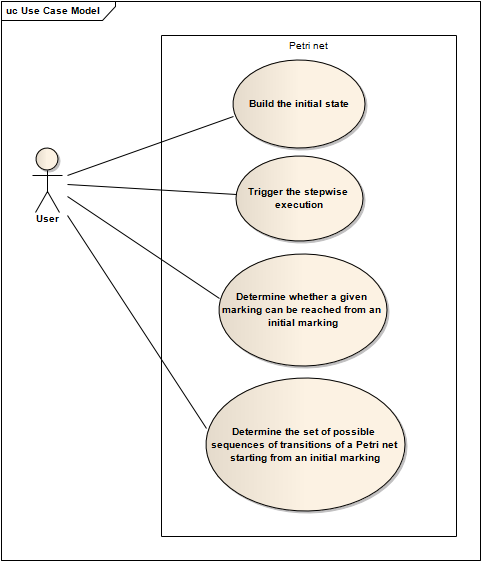
\includegraphics[height= 20cm, width=15cm]{Use_Case_Model.png}

\subsection {Major Use Cases Descriptions}	

\begin{center}
    \begin{tabular}{| l | p{10cm} |}
    \hline
    Scenario & Trigger stepwise execution \\ \hline
    Description & User triggers a transition of the Petri net \\ \hline
    Pre-conditions & 
    \begin{minipage}{10cm}
    \vskip 4pt
    \begin{enumerate}
    	\item The specified transition exists in the Petri net. (\textit{input})
    \end{enumerate}
    \vskip 4pt
    \end{minipage}
    \\ \hline
    Post-conditions & 
    \begin{minipage}{10cm}
    \vskip 4pt
    \begin{enumerate}
    	\item The marking places domain remains unchanged.
    	\item The marking of the Petri net is changed according to the triggered transition. (\textit{output})
    \end{enumerate}
    \vskip 4pt
    \end{minipage} \\ \hline
    Steps &
    \begin{minipage}{10cm}
    \vskip 4pt
    (Unspecified)
    \vskip 4pt
    \end{minipage}
    \\ \hline
    Exceptions & 
    \begin{minipage}{10cm}
    \vskip 4pt
    (Unspecified)
    \vskip 4pt
    \end{minipage}
    \\ \hline
    \end{tabular}
\end{center}


%Reachability%

\begin{center}
    \begin{tabular}{| l | p{10cm} |}
    \hline
    Scenario & Determine marking reachability \\ \hline
    Description &  Determine whether a given marking can be reached from an initial marking \\ \hline
    Pre-conditions & 
    \begin{minipage}{10cm}
    \vskip 4pt
    \begin{enumerate}
    	\item The places of the given marking exist in the Petri net (\textit{input})
    \end{enumerate}
    \vskip 4pt
    \end{minipage}
    \\ \hline
    Post-conditions & 
    \begin{minipage}{10cm}
    \vskip 4pt
    \begin{enumerate}
    \item The state of the Petri net remains unchanged (\textit{final system state})
    \end{enumerate}
    \vskip 4pt
    \end{minipage} \\ \hline
    Steps &
    \begin{minipage}{10cm}
    \vskip 4pt
    (Unspecified)
    \vskip 4pt
    \end{minipage}
    \\ \hline
    Exceptions & 
    \begin{minipage}{10cm}
    \vskip 4pt
    Behaviour is undefined if the Petri net has cycles.
    \vskip 4pt
    \end{minipage}
    \\ \hline
    \end{tabular}
\end{center}

% Set of transitions %

\begin{center}
    \begin{tabular}{| l | p{10cm} |}
    \hline
    Scenario & Get all sequences of transitions \\ \hline
    Description &  Get all sequences of transitions from an initial and target marking \\ \hline
    Pre-conditions & 
    \begin{minipage}{10cm}
    \vskip 4pt
    \begin{enumerate}
    	\item The places of the initial and target markings exist in the Petri net (\textit{input})
    \end{enumerate}
    \vskip 4pt
    \end{minipage}
    \\ \hline
    Post-conditions & 
    \begin{minipage}{10cm}
    \vskip 4pt
    \begin{enumerate}
    \item The state of the Petri net remains unchanged (\textit{final system state})
    \end{enumerate}
    \vskip 4pt
    \end{minipage} \\ \hline
    Steps &
    \begin{minipage}{10cm}
    \vskip 4pt
    (Unspecified)
    \vskip 4pt
    \end{minipage}
    \\ \hline
    Exceptions & 
    \begin{minipage}{10cm}
    \vskip 4pt
    Behaviour is undefined if the Petri net has cycles.
    \vskip 4pt
    \end{minipage}
    \\ \hline
    \end{tabular}
\end{center}

\newpage
\section {Visual UML model}

% Visual UML model  [10%]
% 	A use case diagram, describing the system actors and use cases, with a short description of each actor and use case.
% 	One or more class diagram(s), describing the structure of the VDM++ model, with a short description of each class and type, plus other relevant explanations.

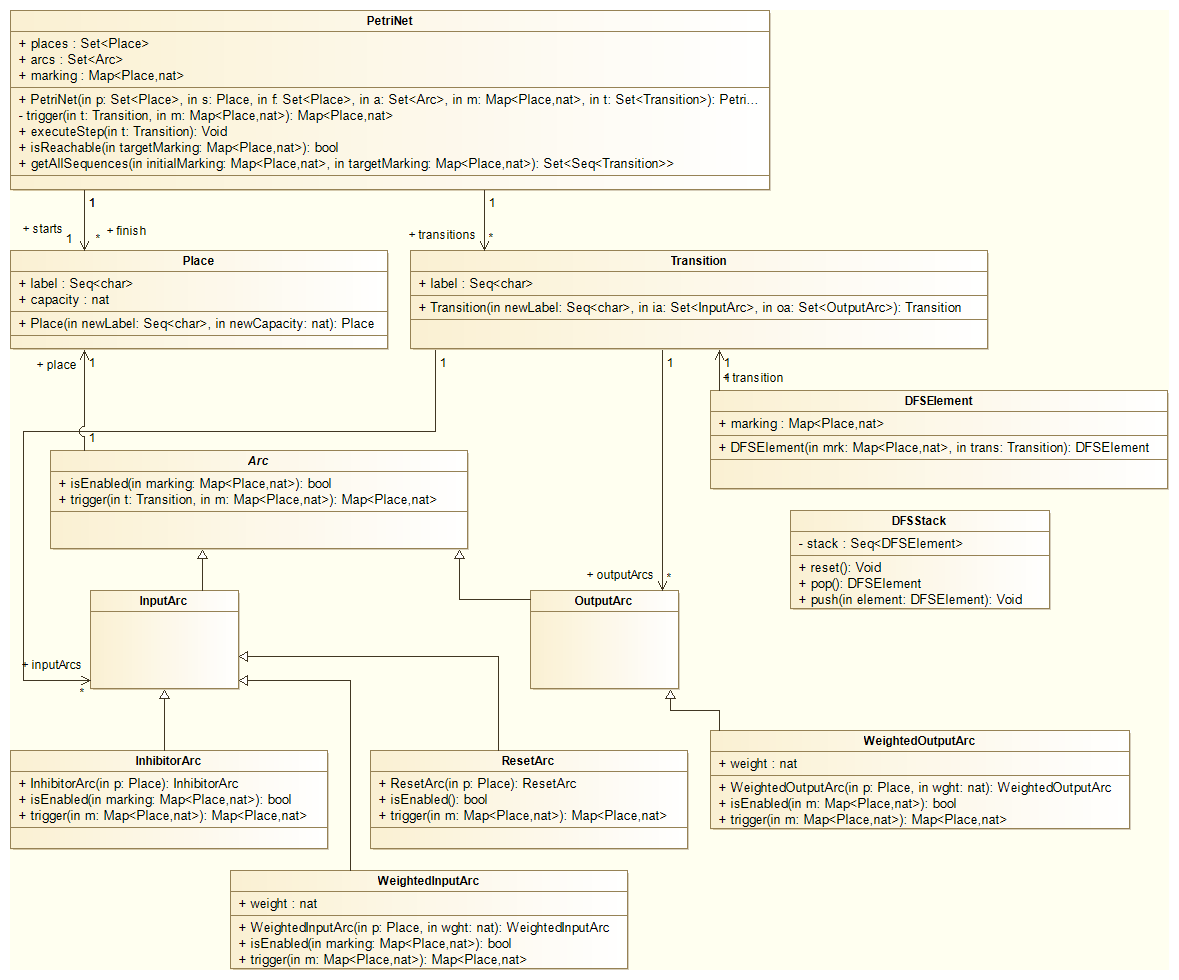
\includegraphics[width=17cm]{class_diagram_full.png}

\newpage 

\section {Formal VDM++ model}
\label{sec:formal_model}

% VDM++ classes, properly commented.
% Needed data types (e.g., String, Date, etc.) should be modeled with types, values and functions.
% Domain entities should be modeled with classes, instance variables and operations.
% You are expected to make adequate usage of the VDM++ types (sets, sequences, maps, etc.) and create a model at a high level of abstraction.
% The model should contain adequate contracts, i.e., invariants, preconditions, and postconditions. Postconditions need only be defined in cases where they are significantly different from the operation or function body.
% During the development of the project, if you foresee that the size of the VDM++ model will be less than 5 pages or more than 10 pages, you should contact your teacher to possibly adjust the scope of the system or the modeling approach being followed.

\subsection{Arc}
\begin{vdmpp}
/*
 * Abstract class to represent arcs between transitions and places
 */
class Arc
  instance variables
    /**
     * Place origin or destination of this arc
     */
    public place: Place
  operations
    /**
     * Returns true if the arc meets all requirements for an 'event' to happen
     *
     * @param marking mapping of places to number of tokens
     * @return boolean
     */
(*@
\label{isEnabled:17}
@*)
    public isEnabled: map Place to nat ==> bool
    isEnabled(marking) == is subclass responsibility;

    /**
     * Modifies the marking at the place of the arc
     *
     * @remark Should only be called if arc is enabled
     * @see isEnabled(marking)
     *
     * @param t transition to be triggered
     * @param m initial marking
     * @return new marking
     */
(*@
\label{trigger:30}
@*)
    public trigger: Transition * map Place to nat ==> map Place to nat
    trigger(t, m) == is subclass responsibility;
    -- pre isEnabled(m);

end Arc

/**
 * Abstract class for all input arcs: arcs from a place to a transition
 */
class InputArc is subclass of Arc

end InputArc

/**
 * Input arc that consumes all tokens at its place
 */
class ResetArc is subclass of InputArc
  operations
    /**
     * ResetArc constructor.
     *
     * @param place place connected to this arc
     */
(*@
\label{ResetArc:53}
@*)
    public ResetArc: Place ==> ResetArc
    ResetArc(p) == (
      place := p;
      return self;
    );

    /**
     * Reset arcs are always enabled
     *
     * @param marking mapping of places to number of tokens
     * @return boolean
     */
(*@
\label{isEnabled:65}
@*)
    public isEnabled: map Place to nat ==> bool
    isEnabled(marking) == (
      return true;
    )
    pre place in set dom marking;

    /**
     * Reset arcs consume all the tokens at the place
     *
     * @remark Should only be called if arc is enabled
     * @see isEnabled(marking)
     *
     * @param t transition to be triggered
     * @param m initial marking
     * @return new marking
     */
(*@
\label{trigger:80}
@*)
    public trigger: Transition * map Place to nat ==> map Place to nat
    trigger(-, m) == (
      dcl newMarking: map Place to nat := m;
      newMarking(place) := 0;
      return newMarking;
    )
    -- pre isEnabled(m)
    pre place in set dom m;

end ResetArc

/**
 * Input arc that is enabled if its place has no tokens
 */
class InhibitorArc is subclass of InputArc
  operations
    /**
     * InhibitorArc constructor.
     *
     * @param place place connected to this arc
     */
(*@
\label{InhibitorArc:100}
@*)
    public InhibitorArc: Place ==> InhibitorArc
    InhibitorArc(p) == (
      place := p;
      return self;
    );

    /**
     * Inhibitor arcs are enabled if their place is empty
     *
     * @param marking mapping of places to number of tokens
     * @return boolean
     */
(*@
\label{isEnabled:112}
@*)
    public isEnabled: map Place to nat ==> bool
    isEnabled(marking) == (
      if marking(place) = 0 then
        return true
      else
        return false;
    )
    pre place in set dom marking;

    /**
     * Inhibitor arcs do not change marking
     *
     * @remark Should only be called if arc is enabled
     * @see isEnabled(marking)
     *
     * @param t transition to be triggered
     * @param m initial marking
     * @return new marking
     */
(*@
\label{trigger:130}
@*)
    public trigger: Transition * map Place to nat ==> map Place to nat
    trigger(-, m) == (
      return m;
    )
    -- pre isEnabled(m)
    pre place in set dom m;

end InhibitorArc

/**
 * Input arc with weight
 */
class WeightedInputArc is subclass of InputArc
  instance variables
    /**
     * Amount of tokens that can 'travel' this arc
     */
    public weight: nat;
  operations
    /**
     * WeightedInputArc constructor.
     *
     * @param place place connected to this arc
     * @param weight capacity of this arc
     */
(*@
\label{WeightedInputArc:154}
@*)
    public WeightedInputArc: Place * nat ==> WeightedInputArc
    WeightedInputArc(p, wght) == (
      place := p;
      weight := wght;
      return self
    );

    /**
     * Weighted input arcs are enabled if the weight
     * is less than the number of tokens of their place
     *
     * @param marking mapping of places to number of tokens
     * @return boolean
     */
(*@
\label{isEnabled:168}
@*)
    public isEnabled: map Place to nat ==> bool
    isEnabled(marking) == (
      return marking(place) >= weight;
    )
    pre place in set dom marking;

    /**
     * Weighted input arcs remove <weight> tokens from their place
     *
     * @remark Should only be called if arc is enabled
     * @see isEnabled(marking)
     *
     * @param t transition to be triggered
     * @param m initial marking
     * @return new marking
     */
(*@
\label{trigger:183}
@*)
    public trigger: Transition * map Place to nat ==> map Place to nat
    trigger(-, m) == (
      dcl newMarking: map Place to nat := m;
      newMarking(place) := newMarking(place) - weight;
      return newMarking;
    )
    -- pre isEnabled(m)
    pre place in set dom m;

end WeightedInputArc

/**
 * Abstract class for all output arcs: arcs from a transtion to a place
 */
class OutputArc is subclass of Arc

end OutputArc

/**
 * Output arc with weight
 */
class WeightedOutputArc is subclass of OutputArc
  instance variables
   /**
    * Amount of tokens that can 'travel' this arc
    */
    public weight: nat;
  operations
    /**
     * WeightedOutputArc constructor.
     *
     * @param place place connected to this arc
     * @param weight capacity of this arc
     */
(*@
\label{WeightedOutputArc:216}
@*)
    public WeightedOutputArc: Place * nat ==> WeightedOutputArc
    WeightedOutputArc(p, wght) == (
      place := p;
      weight := wght;
      return self
    );

    /**
     * Weighted output arcs are enabled if their place
     * capacity is not overrun after moving <weight> tokens
     *
     * @param marking mapping of places to number of tokens
     * @return boolean
     */
(*@
\label{isEnabled:230}
@*)
    public isEnabled: map Place to nat ==> bool
    isEnabled(m) == (
      return m(place) + weight <= place.capacity;
    )
    pre place in set dom m;

    /**
     * Weighted output arcs moves <weight> tokens to their place
     *
     * @remark Should only be called if arc is enabled
     * @see isEnabled(marking)
     *
     * @param t transition to be triggered
     * @param m initial marking
     * @return new marking
     */
(*@
\label{trigger:245}
@*)
    public trigger: Transition * map Place to nat ==> map Place to nat
    trigger(-, m) == (
      dcl newMarking: map Place to nat := m;
      newMarking(place) := newMarking(place) + weight;
      return newMarking;
    )
    -- pre isEnabled(m)
    pre place in set dom m;

end WeightedOutputArc
\end{vdmpp}
\bigskip
\begin{longtable}{|l|r|r|r|}
\hline
Function or operation & Line & Coverage & Calls \\
\hline
\hline
\hyperref[InhibitorArc:100]{InhibitorArc} & 100&100.0\% & 2 \\
\hline
\hyperref[ResetArc:53]{ResetArc} & 53&100.0\% & 2 \\
\hline
\hyperref[WeightedInputArc:154]{WeightedInputArc} & 154&100.0\% & 19 \\
\hline
\hyperref[WeightedOutputArc:216]{WeightedOutputArc} & 216&100.0\% & 24 \\
\hline
\hyperref[isEnabled:112]{isEnabled} & 112&100.0\% & 5 \\
\hline
\hyperref[isEnabled:168]{isEnabled} & 168&100.0\% & 144 \\
\hline
\hyperref[isEnabled:230]{isEnabled} & 230&100.0\% & 100 \\
\hline
\hyperref[isEnabled:65]{isEnabled} & 65&100.0\% & 4 \\
\hline
\hyperref[isEnabled:17]{isEnabled} & 17&100.0\% & 2 \\
\hline
\hyperref[trigger:80]{trigger} & 80&100.0\% & 4 \\
\hline
\hyperref[trigger:183]{trigger} & 183&100.0\% & 83 \\
\hline
\hyperref[trigger:30]{trigger} & 30&100.0\% & 2 \\
\hline
\hyperref[trigger:245]{trigger} & 245&100.0\% & 97 \\
\hline
\hyperref[trigger:130]{trigger} & 130&100.0\% & 2 \\
\hline
\hline
Arc.vdmpp & & 100.0\% & 490 \\
\hline
\end{longtable}

\newpage

\subsection{PetriNet}
\begin{vdmpp}
/**
 * This class represents Petri nets with places, transitions
 * and multiple types of arcs
 */
class PetriNet
  instance variables
    /**
     * set of places (redundant, places are referenced from arcs)
     */
    public places : set of Place := {};

    /**
     * set of arcs (redundant, arcs are referenced from transitions)
     */
    public arcs : set of Arc := {};

    /**
     * set of transitions
     */
    public transitions : set of Transition := {};

    /**
     * state of the Petri net
     * mapping of places to number of tokens
     */
    public marking: map Place to nat := {|->};

    /**
     * single starting place
     */
    public starts : Place;

    /**
     * multiple ending places
     */
    public finish : set of Place := {};

    inv starts in set places;
    inv finish subset places;
    inv forall arc in set arcs & arc.place in set places;
    inv dom marking subset places;
    inv forall transition in set transitions & (
     transition.inputArcs subset arcs and
     transition.outputArcs subset arcs
    );

  operations
    /**
     * PetriNet constructor.
     *
     * @param p set of places
     * @param s start place
     * @param f set of finish places
     * @param a set of arcs
     * @param m initial marking (mapping of places to number of tokens)
     * @param t set of transitions
     */
(*@
\label{PetriNet:57}
@*)
    public PetriNet: set of Place * Place * set of Place * set of Arc *
                     map Place to nat * set of Transition ==> PetriNet
    PetriNet(p, s, f, a, m, t) == (
      atomic(
        places := p;
        starts := s;
        finish := f;
        arcs := a;
        marking := m;
        transitions := t;
      )
      return self;
    )
    pre dom m = p and
      s in set p and
      f subset p and
      forall a1 in set a & a1.place in set p and
      forall t1 in set t & (
       forall a2 in set t1.inputArcs & a2 in set a and
       forall a3 in set t1.outputArcs & a3 in set a
      );

    /**
     * Triggers given transition and returns the new state of the Petri net.
     *
     * @remark The internal state of the Petri net is not changed by this
     *         method. For that intention, use executeStep instead.
     *
     * @param t transition to be triggered
     * @param m marking (mapping of places to number of tokens)
     * @return  new marking representing the new state of the Petri net.
     *          It may or may not have been modified, depending if
     *          the transition was actually triggered (i.e all conditions
     *          at the arcs have been met).
     */
(*@
\label{trigger:90}
@*)
    private trigger: Transition * map Place to nat ==> map Place to nat
    trigger(t, m) == (
      dcl newMarking: map Place to nat := m;

      for all arc in set t.inputArcs do (
        if not arc.isEnabled(newMarking) then
          return m;
        newMarking := arc.trigger(t, newMarking);
      );

      for all arc in set t.outputArcs do (
        if not arc.isEnabled(newMarking) then
          return m;
        newMarking := arc.trigger(t, newMarking);
      );

      return newMarking;
    )
    pre t in set transitions and dom m subset places
    post dom RESULT subset places;

    /**
     * Triggers given transition and changes marking accordingly.
     *
     * @see trigger(t, m)
     *
     * @param t transition to be triggered
     * @return  nothing
     */
(*@
\label{executeStep:119}
@*)
    public executeStep: Transition ==> ()
    executeStep(t) == (
      marking := trigger(t, marking);
    )
    pre t in set transitions;

    /**
     * Verifies if a given marking is reachable from current state.
     *
     * Reachability definition (@wikipedia): "Given a computational
     * (potentially infinite state) system with a set of allowed rules
     * or transformations, decide whether a certain state of a system is
     * reachable from a given initial state of the system."
     *
     * @remark The behaviour is undefined if the Petri net is cyclic
     *
     * @param targetMarking marking (mapping of places to number of tokens)
     * @return boolean
     */
(*@
\label{isReachable:138}
@*)
    public isReachable: map Place to nat ==> bool
    isReachable(targetMarking) == (
      dcl stack: DFSStack := new DFSStack();
      dcl currentInputMarking: map Place to nat := marking;
      dcl currentOutputMarking: map Place to nat := marking;
      dcl previousMarkings: set of map Place to nat := {};

      stack.push(new DFSElement(marking, new Transition("Start", { }, { })));

      while not stack.empty() do (

        currentInputMarking := stack.pop().marking;

        for all transition in set transitions do (

          currentOutputMarking := trigger(transition, currentInputMarking);

          /* if target marking is found */
          if (currentOutputMarking = targetMarking) then return true;

          /* if marking is not already explored */
          if (currentOutputMarking not in set previousMarkings) then (
            stack.push(new DFSElement(currentOutputMarking, transition));
            previousMarkings := previousMarkings union {currentOutputMarking};
          )
        );

      );

      return false;
    )
    pre dom targetMarking subset places;

    /**
     * Get all sequences of transitions from an initial marking and
     * a target marking.
     *
     * @remark The behaviour is undefined if the Petri net is cyclic
     *
     * @param initialMarking initial marking (mapping of places to number of tokens)
     * @param targetMarking final marking (mapping of places to number of tokens)
     * @return set of seq of transitions
     */
(*@
\label{getAllSequences:181}
@*)
    public getAllSequences: map Place to nat * map Place to nat ==> set of seq of Transition
    getAllSequences(initialMarking, targetMarking) == (
      dcl stack: DFSStack := new DFSStack();
      dcl currentDFSElement: DFSElement;
      dcl currentInputMarking: map Place to nat := initialMarking;
      dcl currentTransition: Transition;
      dcl currentOutputMarking: map Place to nat := initialMarking;
      dcl previousMarkings: set of map Place to nat := {};
      dcl transitionSeqs: set of seq of Transition := {};
      dcl sequencePath: seq of Transition := [];
      dcl newMarkingsGenerated: bool := false;
      dcl dummyTransition: Transition := new Transition("Start", { }, { });

      stack.push(new DFSElement(initialMarking, dummyTransition));

      while not stack.empty() do (

        currentDFSElement := stack.pop();
        currentTransition := currentDFSElement.transition;
        currentInputMarking := currentDFSElement.marking;

        newMarkingsGenerated := false;

        if (currentTransition <> dummyTransition) then
          sequencePath := [currentTransition] ^ sequencePath;

        for all transition in set transitions do (

          currentOutputMarking := trigger(transition, currentInputMarking);

          /* if target marking is found */
          if (currentOutputMarking = targetMarking and
           currentOutputMarking <> currentInputMarking and
           currentOutputMarking not in set previousMarkings) then (
            if (len sequencePath <> 0) then (
              transitionSeqs := transitionSeqs union {sequencePath ^ [transition]};
            );
          );

          /* if marking is not already explored */
          if (currentOutputMarking not in set previousMarkings) then (
            newMarkingsGenerated := true;
            stack.push(new DFSElement(currentOutputMarking, transition));
            previousMarkings := previousMarkings union {currentOutputMarking};
          );

          /* reached a dead end, remove sequence from path, a backtracking will occur */
          if (not newMarkingsGenerated) then (
            if (len sequencePath > 0) then
              sequencePath := tl sequencePath;
          );

        );

      );

      return transitionSeqs;
    )
    pre dom initialMarking subset places and dom targetMarking subset places;

end PetriNet
\end{vdmpp}
\bigskip
\begin{longtable}{|l|r|r|r|}
\hline
Function or operation & Line & Coverage & Calls \\
\hline
\hline
\hyperref[PetriNet:57]{PetriNet} & 57&100.0\% & 9 \\
\hline
\hyperref[executeStep:119]{executeStep} & 119&100.0\% & 20 \\
\hline
\hyperref[getAllSequences:181]{getAllSequences} & 181&100.0\% & 3 \\
\hline
\hyperref[isReachable:138]{isReachable} & 138&100.0\% & 18 \\
\hline
\hyperref[trigger:90]{trigger} & 90&100.0\% & 142 \\
\hline
\hline
PetriNet.vdmpp & & 100.0\% & 192 \\
\hline
\end{longtable}

\newpage

\subsection{Place}
\begin{vdmpp}
/**
 * Place of a Petri net with a maximum capacity
 */
class Place
  instance variables
    /**
     * Name of the place (debug/cosmetic purposes)
     */
    public label: seq of char;

    /**
     * Maximum number of tokens that this place can hold
     */
    public capacity: nat;

  operations
    /**
     * Place constructors.
     *
     * @param newLabel description of the place
     * @param newCapacity capacity of the place
     */
(*@
\label{Place:23}
@*)
    public Place: seq of char * nat ==> Place
    Place(newLabel, newCapacity) == (
      label := newLabel;
      capacity := newCapacity;
      return self
    )
    pre newCapacity > 0;
end Place
\end{vdmpp}
\bigskip
\begin{longtable}{|l|r|r|r|}
\hline
Function or operation & Line & Coverage & Calls \\
\hline
\hline
\hyperref[Place:23]{Place} & 23&100.0\% & 27 \\
\hline
\hline
Place.vdmpp & & 100.0\% & 27 \\
\hline
\end{longtable}

\newpage

\subsection{Transition}
\begin{vdmpp}
/**
 * Transition of a Petri net
 */
class Transition
  instance variables
    /**
     * Name of the transition (debug/cosmetic purposes)
     */
    public label: seq of char;

    /**
     * Set of all input arcs to this transition
     */
    public inputArcs: set of InputArc;

    /**
     * Set of all output arcs from this transition
     */
    public outputArcs: set of OutputArc;

  operations
    /**
     * Transition constructors.
     *
     * @param newLabel description of the transition
     * @param ia set of connected input places
     * @param oa set of connected output places
     */
(*@
\label{Transition:29}
@*)
    public Transition: seq of char * set of InputArc * set of OutputArc ==> Transition
    Transition(newLabel, ia, oa) == (
      label := newLabel;
      inputArcs := ia;
      outputArcs := oa;
      return self;
    );
end Transition
\end{vdmpp}
\bigskip
\begin{longtable}{|l|r|r|r|}
\hline
Function or operation & Line & Coverage & Calls \\
\hline
\hline
\hyperref[Transition:29]{Transition} & 29&100.0\% & 38 \\
\hline
\hline
Transition.vdmpp & & 100.0\% & 38 \\
\hline
\end{longtable}

\newpage

\subsection{DFSStack}
\begin{vdmpp}
class DFSStack
  instance variables
    stack: seq of DFSElement := [];
  operations
(*@
\label{reset:5}
@*)
    public reset: () ==> ()
    reset() ==
      stack := [];
(*@
\label{pop:8}
@*)
    public pop: () ==> DFSElement
    pop() ==
      def res = hd stack in
      (stack := tl stack;
      return res)
    pre stack <> [];

(*@
\label{push:15}
@*)
    public push: DFSElement ==> ()
    push(element) == (
      stack := [element] ^ stack;
    );

(*@
\label{empty:20}
@*)
    public empty: () ==> bool
    empty() == (
      return len stack = 0
    );

end DFSStack

class DFSElement
  instance variables
    public marking: map Place to nat;
    public transition: Transition;
  operations
(*@
\label{DFSElement:32}
@*)
    public DFSElement: map Place to nat * Transition ==> DFSElement
    DFSElement(mrk, trans) == (
      marking := mrk;
      transition := trans;
      return self;
    );
end DFSElement
\end{vdmpp}
\bigskip
\begin{longtable}{|l|r|r|r|}
\hline
Function or operation & Line & Coverage & Calls \\
\hline
\hline
\hyperref[DFSElement:32]{DFSElement} & 32&100.0\% & 55 \\
\hline
\hyperref[empty:20]{empty} & 20&100.0\% & 59 \\
\hline
\hyperref[pop:8]{pop} & 8&100.0\% & 53 \\
\hline
\hyperref[push:15]{push} & 15&100.0\% & 55 \\
\hline
\hyperref[reset:5]{reset} & 5&0.0\% & 0 \\
\hline
\hline
DFSStack.vdmpp & & 100.0\% & 22 \\
\hline
\end{longtable}

\newpage

\section {Model validation}

% Model validation (i.e., testing) [20%]
% 	VDM++ test classes, containing adequate and thorough test cases defined by means of traces or operations.
% 	Optionally, figures of examples exercised in the test cases.
% 	Evidences of test results (passed/failed). A printscreen may be sufficient.
% 	Code coverage information (it is sufficient to present the system classes mentioned in 4 painted with coverage information). Ideally, 100% coverage should be achieved.
% 	Requirements traceability relationship between test cases and requirements. Ideally, 100% requirements coverage should be achieved. It may be sufficient to indicate in comments for each test case the requirements that are exercised.

\subsection{MyTestCase}
\begin{vdmpp}
/*
 * Superclass for test classes, simpler but more practical than VDMUnit`TestCase.
 * For proper use, you have to do: New -> Add VDM Library -> IO.
 * JPF, FEUP, MFES, 2014/15.
 */
class MyTestCase
operations

  /**
   * Simulates assertion checking by reducing it to pre-condition checking.
   * If 'arg' does not hold, a pre-condition violation will be signaled.
   */
(*@
\label{assertTrue:13}
@*)
  protected assertTrue: bool ==> ()
  assertTrue(arg) ==
    return
  pre arg;

  /**
   * Simulates assertion checking by reducing it to post-condition checking.
   * If values are not equal, prints a message in the console and generates
   * a post-conditions violation.
   */
(*@
\label{assertEqual:23}
@*)
  protected assertEqual: ? * ? ==> ()
  assertEqual(expected, actual) ==
    if expected <> actual then (
      IO`print("Actual value (");
      IO`print(actual);
      IO`print(") different from expected (");
      IO`print(expected);
      IO`println(")\n")
    )
  post expected = actual

end MyTestCase
\end{vdmpp}
\bigskip
\begin{longtable}{|l|r|r|r|}
\hline
Function or operation & Line & Coverage & Calls \\
\hline
\hline
\hyperref[assertEqual:23]{assertEqual} & 23&38.8\% & 43 \\
\hline
\hyperref[assertTrue:13]{assertTrue} & 13&100.0\% & 18 \\
\hline
\hline
MyTestCase.vdmpp & & 45.0\% & 61 \\
\hline
\end{longtable}

\newpage

\subsection{TestArc}
\begin{vdmpp}
class TestArc is subclass of MyTestCase

operations
(*@
\label{testConstructors:4}
@*)
  public testConstructors: () ==> ()
  testConstructors() == (
    IO`println("\t\t test constructor");
    let p = new Place(),
     wia = new WeightedInputArc(p, 1),
     ra = new ResetArc(p),
     ia = new InhibitorArc(p),
     woa = new WeightedOutputArc(p, 2) in (
      assertEqual(1, wia.weight);
      assertEqual(2, woa.weight);
      assertEqual(p, wia.place);
      assertEqual(p, woa.place);
      assertEqual(p, ra.place);
      assertEqual(p, ia.place);
    );
  );

  /**
   * Entry point that runs all tests with valid inputs (no test should fail)
   */
(*@
\label{testAll:24}
@*)
  public testAll: () ==> ()
  testAll() == (
    IO`println("\t arc tests");
    testConstructors();
  );

end TestArc
\end{vdmpp}
\bigskip
\begin{longtable}{|l|r|r|r|}
\hline
Function or operation & Line & Coverage & Calls \\
\hline
\hline
\hyperref[testAll:24]{testAll} & 24&100.0\% & 1 \\
\hline
\hyperref[testConstructors:4]{testConstructors} & 4&100.0\% & 1 \\
\hline
\hline
TestArc.vdmpp & & 100.0\% & 2 \\
\hline
\end{longtable}

\newpage

\subsection{TestPetriNet}
\begin{vdmpp}
class TestPetriNet is subclass of MyTestCase

operations
  /**
   * Requirements: R1, R2.3, R2.4, R3, R4, R5
   */
(*@
\label{testElevator1Example:4}
@*)
(*@
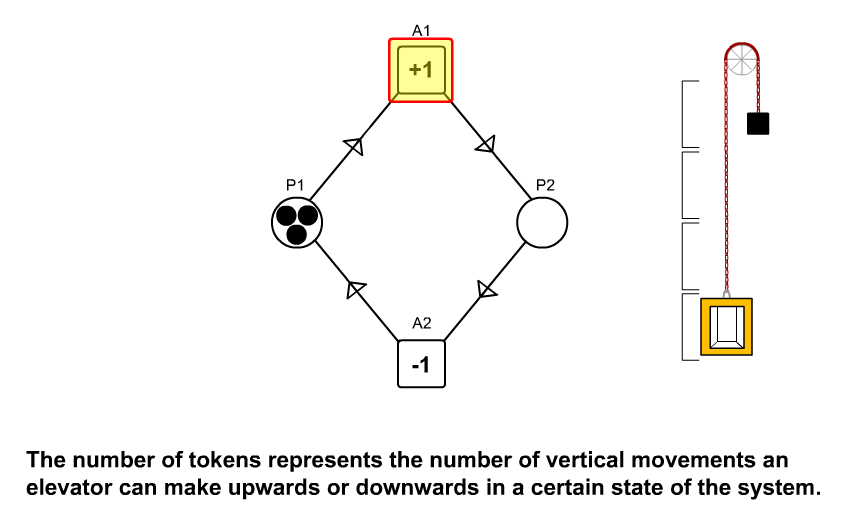
\includegraphics[width=5cm]{specification/elevator1.png}
@*)
  public testElevator1Example: () ==> ()
  testElevator1Example() == (
    /* http://www.informatik.uni-hamburg.de/TGI/PetriNets/introductions/aalst/elevator1.swf */
    IO`println("\t\t test elevator 1");
    let p1 = new Place("P1", 3),
     p2 = new Place("P2", 3),
     a1i = new WeightedInputArc(p1, 1),
     a1o = new WeightedOutputArc(p2, 1),
     a2i = new WeightedInputArc(p2, 1),
     a2o = new WeightedOutputArc(p1, 1),
     t1 = new Transition("+1", { a1i }, { a1o }),
     t2 = new Transition("-1", { a2i }, { a2o }),

     places = { p1, p2 },
     arcs = { a1i, a1o, a2i, a2o },
     marking = { p1 |-> 3, p2 |-> 0 },
     transitions = { t1, t2 },

     petriNet = new PetriNet(places, p1, {}, arcs, marking, transitions) in (

      assertEqual({ p1 |-> 3, p2 |-> 0 }, petriNet.marking);

      /* Test reachability of the markings before step execution */
      assertTrue(petriNet.isReachable({ p1 |-> 2, p2 |-> 1 }));
      assertTrue(petriNet.isReachable({ p1 |-> 1, p2 |-> 2 }));
      assertTrue(petriNet.isReachable({ p1 |-> 0, p2 |-> 3 }));
      assertTrue(not petriNet.isReachable({ p1 |-> 4, p2 |-> 5 }));

      assertEqual({}, petriNet.getAllSequences(
        { p1 |-> 3, p2 |-> 0 },{ p1 |-> 4, p2 |-> 5 })
      );
      assertEqual({[t1, t1]}, petriNet.getAllSequences(
        { p1 |-> 3, p2 |-> 0 }, { p1 |-> 1, p2 |-> 2 })
      );
      assertEqual({[t1, t1, t1]}, petriNet.getAllSequences(
        { p1 |-> 3, p2 |-> 0 }, { p1 |-> 0, p2 |-> 3 })
      );

      /* Test stepwise execution of the petri net */
      petriNet.executeStep(t1);
      assertEqual({ p1 |-> 2, p2 |-> 1 }, petriNet.marking);

      petriNet.executeStep(t1);
      assertEqual({ p1 |-> 1, p2 |-> 2 }, petriNet.marking);

      petriNet.executeStep(t1);
      assertEqual({ p1 |-> 0, p2 |-> 3 }, petriNet.marking);

      petriNet.executeStep(t2);
      assertEqual({ p1 |-> 1, p2 |-> 2 }, petriNet.marking);

      petriNet.executeStep(t1);
      assertEqual({ p1 |-> 0, p2 |-> 3 }, petriNet.marking);
    );
  );

  /**
   * Requirements: R1, R2.3, R2.4, R3, R4, R5
   */
(*@
\label{testElevator2Example:60}
@*)
(*@
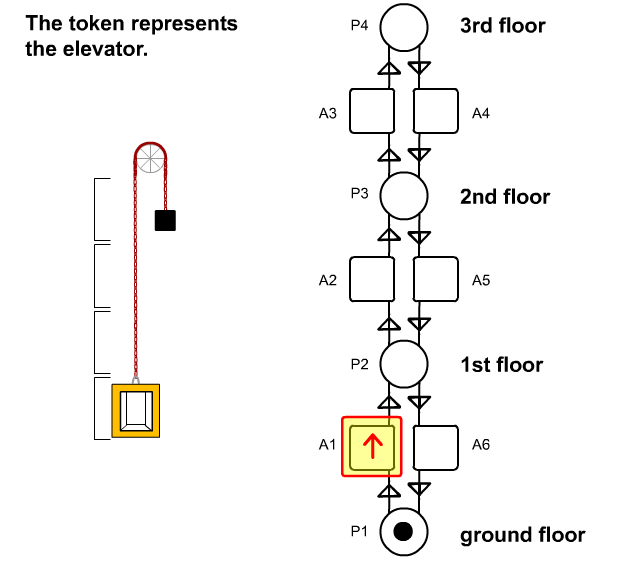
\includegraphics[width=5cm]{specification/elevator2.png}
@*)
  public testElevator2Example: () ==> ()
  testElevator2Example() == (
    /* http://www.informatik.uni-hamburg.de/TGI/PetriNets/introductions/aalst/elevator2.swf */
    IO`println("\t\t test elevator 2");
    let p1 = new Place("ground floor", 1),
     p2 = new Place("1st floor", 1),
     p3 = new Place("2nd floor", 1),
     p4 = new Place("3rd floor", 1),
     a1i = new WeightedInputArc(p1, 1),
     a1o = new WeightedOutputArc(p2, 1),
     a2i = new WeightedInputArc(p2, 1),
     a2o = new WeightedOutputArc( p3, 1),
     a3i = new WeightedInputArc(p3, 1),
     a3o = new WeightedOutputArc(p4, 1),
     a4i = new WeightedInputArc(p4, 1),
     a4o = new WeightedOutputArc(p3, 1),
     a5i = new WeightedInputArc(p3, 1),
     a5o = new WeightedOutputArc(p2, 1),
     a6i = new WeightedInputArc(p2, 1),
     a6o = new WeightedOutputArc(p1, 1),
     t1 = new Transition("A1", { a1i }, { a1o }),
     t2 = new Transition("A2", { a2i }, { a2o }),
     t3 = new Transition("A3", { a3i }, { a3o }),
     t4 = new Transition("A4", { a4i }, { a4o }),
     t5 = new Transition("A5", { a5i }, { a5o }),
     t6 = new Transition("A6", { a6i }, { a6o }),

     places = { p1, p2, p3, p4 },
     arcs = { a1i, a1o, a2i, a2o, a3i, a3o, a4i, a4o, a5i, a5o, a6i, a6o },
     marking = { p1 |-> 1, p2 |-> 0, p3 |-> 0, p4 |-> 0 },
     transitions = { t1, t2, t3, t4, t5, t6 },

     petriNet = new PetriNet(places, p1, {}, arcs, marking, transitions) in (

      /* Test reachability before stepwise execution */
      assertTrue(petriNet.isReachable({ p1 |-> 1, p2 |-> 0, p3 |-> 0, p4 |-> 0 }));
      assertTrue(petriNet.isReachable({ p1 |-> 0, p2 |-> 1, p3 |-> 0, p4 |-> 0 }));
      assertTrue(petriNet.isReachable({ p1 |-> 0, p2 |-> 1, p3 |-> 0, p4 |-> 0 }));

      assertEqual({ p1 |-> 1, p2 |-> 0, p3 |-> 0, p4 |-> 0 }, petriNet.marking);

      /* Test stepwise execution of the Petri net */
      petriNet.executeStep(t1); /* valid */
      assertEqual({ p1 |-> 0, p2 |-> 1, p3 |-> 0, p4 |-> 0 }, petriNet.marking);

      petriNet.executeStep(t2); /* valid */
      assertEqual({ p1 |-> 0, p2 |-> 0, p3 |-> 1, p4 |-> 0 }, petriNet.marking);

      petriNet.executeStep(t5); /* valid */
      assertEqual({ p1 |-> 0, p2 |-> 1, p3 |-> 0, p4 |-> 0 }, petriNet.marking);

      let previousMarking = petriNet.marking in (
        petriNet.executeStep(t1); /* not valid, no marking change */
        assertEqual(previousMarking, petriNet.marking);
      )
    );
  );

  /**
   * Requirements: R1, R2.3, R2.4, R3, R4, R5
   */
(*@
\label{testElevator3Example:118}
@*)
(*@
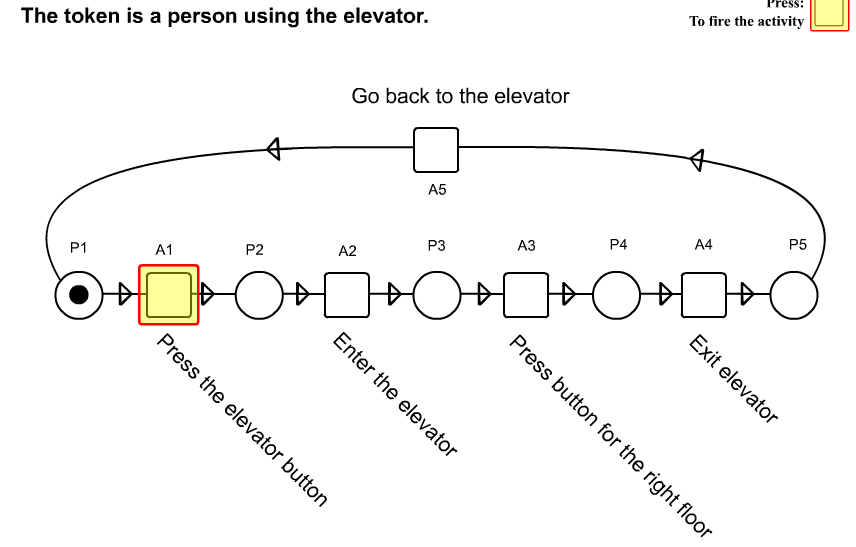
\includegraphics[width=5cm]{specification/elevator3.png}
@*)
  public testElevator3Example: () ==> ()
  testElevator3Example() == (
    /* http://www.informatik.uni-hamburg.de/TGI/PetriNets/introductions/aalst/elevator3.swf */
    IO`println("\t\t test elevator 3");
    let p1 = new Place("p1", 1),
     p2 = new Place("p2", 1),
     p3 = new Place("p3", 1),
     p4 = new Place("p4", 1),
     p5 = new Place("p5", 1),
     a1i = new WeightedInputArc(p1,  1),
     a1o = new WeightedOutputArc(p2, 1),
     a2i = new WeightedInputArc(p2, 1),
     a2o = new WeightedOutputArc(p3, 1),
     a3i = new WeightedInputArc(p3, 1),
     a3o = new WeightedOutputArc(p4, 1),
     a4i = new WeightedInputArc(p4, 1),
     a4o = new WeightedOutputArc(p5, 1),
     a5i = new WeightedInputArc(p5, 1),
     a5o = new WeightedOutputArc(p1, 1),
     t1 = new Transition("A1 - Press the elevator button", { a1i }, { a1o }),
     t2 = new Transition("A2 - Enter the elevator", { a2i }, { a2o }),
     t3 = new Transition("A3 - Press button for the right floor", { a3i }, { a3o }),
     t4 = new Transition("A4 - Exit elevator", { a4i }, { a4o }),
     t5 = new Transition("A5 - Go back to the elevator", { a5i }, { a5o }),

     places = { p1, p2, p3, p4, p5 },
     arcs = { a1i, a1o, a2i, a2o, a3i, a3o, a4i, a4o, a5i, a5o },
     marking = { p1 |-> 1, p2 |-> 0, p3 |-> 0, p4 |-> 0, p5 |-> 0 },
     transitions = { t1, t2, t3, t4, t5 },

     petriNet = new PetriNet(places, p1, {}, arcs, marking, transitions) in (

      /* Test reachability before stepwise execution */
      assertTrue(petriNet.isReachable({ p1 |-> 1, p2 |-> 0, p3 |-> 0, p4 |-> 0, p5 |-> 0 }));
      assertTrue(petriNet.isReachable({ p1 |-> 0, p2 |-> 1, p3 |-> 0, p4 |-> 0, p5 |-> 0 }));
      assertTrue(petriNet.isReachable({ p1 |-> 0, p2 |-> 0, p3 |-> 1, p4 |-> 0, p5 |-> 0 }));
      assertTrue(petriNet.isReachable({ p1 |-> 0, p2 |-> 0, p3 |-> 0, p4 |-> 1, p5 |-> 0 }));
      assertTrue(petriNet.isReachable({ p1 |-> 0, p2 |-> 0, p3 |-> 0, p4 |-> 0, p5 |-> 1 }));

      assertEqual({ p1 |-> 1, p2 |-> 0, p3 |-> 0, p4 |-> 0, p5 |-> 0 }, petriNet.marking);

      /* Test stepwise execution of the petri net */
      petriNet.executeStep(t1); /* valid */
      assertEqual({ p1 |-> 0, p2 |-> 1, p3 |-> 0, p4 |-> 0, p5 |-> 0 }, petriNet.marking);

      petriNet.executeStep(t2); /* valid */
      assertEqual({ p1 |-> 0, p2 |-> 0, p3 |-> 1, p4 |-> 0, p5 |-> 0 }, petriNet.marking);

      petriNet.executeStep(t3); /* valid */
      assertEqual({ p1 |-> 0, p2 |-> 0, p3 |-> 0, p4 |-> 1, p5 |-> 0 }, petriNet.marking);

      petriNet.executeStep(t4); /* valid */
      assertEqual({ p1 |-> 0, p2 |-> 0, p3 |-> 0, p4 |-> 0, p5 |-> 1 }, petriNet.marking);

      petriNet.executeStep(t5); /* valid */
      assertEqual({ p1 |-> 1, p2 |-> 0, p3 |-> 0, p4 |-> 0, p5 |-> 0 }, petriNet.marking);

    );
  );

  /**
   * Requirements: R1, R2.2, R2.3, R2.4, R3, R4
   */
(*@
\label{testSimpleInhibitorArc:178}
@*)
(*@
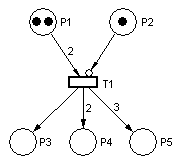
\includegraphics[width=5cm]{specification/simpleinhibitorarc.png}
@*)
  public testSimpleInhibitorArc: () ==> ()
  testSimpleInhibitorArc() == (
    /* http://www.techfak.uni-bielefeld.de/~mchen/BioPNML/Intro/pnfaq_files/image005.gif */
    IO`println("\t\t test simple inhibitor arc");
    let p1 = new Place("P1", 2),
     p2 = new Place("P2", 1),
     p3 = new Place("P3", 1),
     p4 = new Place("P4", 3),
     p5 = new Place("P5", 4),
     ia1 = new WeightedInputArc(p1,  2),
     ia2 = new InhibitorArc(p2),
     oa1 = new WeightedOutputArc(p3, 1),
     oa2 = new WeightedOutputArc(p4, 2),
     oa3 = new WeightedOutputArc(p5, 3),
     t1 = new Transition("T1", { ia1, ia2 }, { oa1, oa2, oa3 }),

     places = { p1, p2, p3, p4, p5 },
     arcs = { ia1, ia2, oa1, oa2, oa3 },
     marking1 = { p1 |-> 2, p2 |-> 1, p3 |-> 0, p4 |-> 0, p5 |-> 0 },
     marking2 = { p1 |-> 2, p2 |-> 0, p3 |-> 0, p4 |-> 0, p5 |-> 0 },
     transitions = { t1 },

     petriNet1 = new PetriNet(places, p1, {}, arcs, marking1, transitions),
     petriNet2 = new PetriNet(places, p1, {}, arcs, marking2, transitions) in (

      assertEqual({ p1 |-> 2, p2 |-> 1, p3 |-> 0, p4 |-> 0, p5 |-> 0 }, petriNet1.marking);
      assertEqual({ p1 |-> 2, p2 |-> 0, p3 |-> 0, p4 |-> 0, p5 |-> 0 }, petriNet2.marking);

      assertTrue(not petriNet1.isReachable(
        { p1 |-> 0, p2 |-> 0, p3 |-> 1, p4 |-> 2, p5 |-> 3 })
      );
      assertTrue( petriNet2.isReachable(
        { p1 |-> 0, p2 |-> 0, p3 |-> 1, p4 |-> 2, p5 |-> 3 })
      );

      petriNet1.executeStep(t1); /* should not trigger */
      petriNet2.executeStep(t1); /* should trigger */

      assertEqual({ p1 |-> 2, p2 |-> 1, p3 |-> 0, p4 |-> 0, p5 |-> 0 }, petriNet1.marking);
      assertEqual({ p1 |-> 0, p2 |-> 0, p3 |-> 1, p4 |-> 2, p5 |-> 3 }, petriNet2.marking);
    );
  );

  /**
   * Requirements: R1, R2.1, R2.3, R2.4, R3, R4
   */
(*@
\label{testSimpleResetArc:221}
@*)
(*@
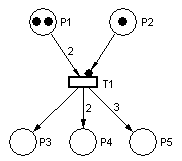
\includegraphics[width=5cm]{specification/simpleresetarc.png}
@*)
  public testSimpleResetArc: () ==> ()
  testSimpleResetArc() == (
    /* http://www.techfak.uni-bielefeld.de/~mchen/BioPNML/Intro/pnfaq_files/image003.gif (mod.) */
    IO`println("\t\t test simple reset arc");
    let p1 = new Place("P1", 2),
     p2 = new Place("P2", 1),
     p3 = new Place("P3", 1),
     p4 = new Place("P4", 3),
     p5 = new Place("P5", 4),
     ia1 = new WeightedInputArc(p1,  2),
     ia2 = new ResetArc(p2),
     oa1 = new WeightedOutputArc(p3, 1),
     oa2 = new WeightedOutputArc(p4, 2),
     oa3 = new WeightedOutputArc(p5, 3),
     t1 = new Transition("T1", { ia1, ia2 }, { oa1, oa2, oa3 }),

     places = { p1, p2, p3, p4, p5 },
     arcs = { ia1, ia2, oa1, oa2, oa3 },
     marking1 = { p1 |-> 2, p2 |-> 5, p3 |-> 0, p4 |-> 0, p5 |-> 0 },
     marking2 = { p1 |-> 2, p2 |-> 0, p3 |-> 0, p4 |-> 0, p5 |-> 0 },
     transitions = { t1 },

     petriNet1 = new PetriNet(places, p1, {}, arcs, marking1, transitions),
     petriNet2 = new PetriNet(places, p1, {}, arcs, marking2, transitions) in (

      assertEqual({ p1 |-> 2, p2 |-> 5, p3 |-> 0, p4 |-> 0, p5 |-> 0 }, petriNet1.marking);
      assertEqual({ p1 |-> 2, p2 |-> 0, p3 |-> 0, p4 |-> 0, p5 |-> 0 }, petriNet2.marking);

      assertTrue(petriNet1.isReachable({ p1 |-> 0, p2 |-> 0, p3 |-> 1, p4 |-> 2, p5 |-> 3 }));
      assertTrue(petriNet2.isReachable({ p1 |-> 0, p2 |-> 0, p3 |-> 1, p4 |-> 2, p5 |-> 3 }));

      petriNet1.executeStep(t1); /* should trigger */
      petriNet2.executeStep(t1); /* should trigger */

      assertEqual({ p1 |-> 0, p2 |-> 0, p3 |-> 1, p4 |-> 2, p5 |-> 3 }, petriNet1.marking);
      assertEqual({ p1 |-> 0, p2 |-> 0, p3 |-> 1, p4 |-> 2, p5 |-> 3 }, petriNet2.marking);
    );
  );

  /**
   * Requirements: R1, R2.3, R2.4, R3, R4
   */
(*@
\label{testSimpleCapacityArc:260}
@*)
(*@
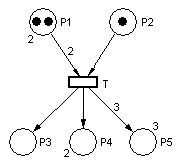
\includegraphics[width=5cm]{specification/simplecapacityarc.png}
@*)
  public testSimpleCapacityArc: () ==> ()
  testSimpleCapacityArc() == (
    /* http://www.techfak.uni-bielefeld.de/~mchen/BioPNML/Intro/pnfaq_files/image003.gif (mod.) */
    IO`println("\t\t test simple capacity arc");
    let p1 = new Place("P1", 2),
     p2 = new Place("P2", 1),
     p3 = new Place("P3", 1),
     p4 = new Place("P4", 2),
     p5 = new Place("P5", 3),
     ia1 = new WeightedInputArc(p1,  2),
     ia2 = new WeightedInputArc(p2,  1),
     oa1 = new WeightedOutputArc(p3, 1),
     oa2 = new WeightedOutputArc(p4, 2),
     oa3 = new WeightedOutputArc(p5, 3),
     t1 = new Transition("T1", { ia1, ia2 }, { oa1, oa2, oa3 }),

     places = { p1, p2, p3, p4, p5 },
     arcs = { ia1, ia2, oa1, oa2, oa3 },
     marking1 = { p1 |-> 2, p2 |-> 1, p3 |-> 0, p4 |-> 0, p5 |-> 3 },
     marking2 = { p1 |-> 2, p2 |-> 1, p3 |-> 0, p4 |-> 0, p5 |-> 0 },
     transitions = { t1 },

     petriNet1 = new PetriNet(places, p1, {}, arcs, marking1, transitions),
     petriNet2 = new PetriNet(places, p1, {}, arcs, marking2, transitions) in (

      assertEqual({ p1 |-> 2, p2 |-> 1, p3 |-> 0, p4 |-> 0, p5 |-> 3 }, petriNet1.marking);
      assertEqual({ p1 |-> 2, p2 |-> 1, p3 |-> 0, p4 |-> 0, p5 |-> 0 }, petriNet2.marking);

      assertTrue(not petriNet1.isReachable(
        { p1 |-> 0, p2 |-> 0, p3 |-> 1, p4 |-> 2, p5 |-> 3 })
      );
      assertTrue(petriNet2.isReachable(
        { p1 |-> 0, p2 |-> 0, p3 |-> 1, p4 |-> 2, p5 |-> 3 })
      );

      petriNet1.executeStep(t1); /* should not trigger */
      petriNet2.executeStep(t1); /* should trigger */

      assertEqual({ p1 |-> 2, p2 |-> 1, p3 |-> 0, p4 |-> 0, p5 |-> 3 }, petriNet1.marking);
      assertEqual({ p1 |-> 0, p2 |-> 0, p3 |-> 1, p4 |-> 2, p5 |-> 3 }, petriNet2.marking);
    );
  );

  /* Entry point that runs all tests with valid inputs */
(*@
\label{testAll:304}
@*)
  public testAll: () ==> ()
  testAll() == (
    IO`println("\t petrinet tests");
    testElevator1Example();
    testElevator2Example();
    testElevator3Example();
    testSimpleInhibitorArc();
    testSimpleResetArc();
    testSimpleCapacityArc();
  );

end TestPetriNet
\end{vdmpp}
\bigskip
\begin{longtable}{|l|r|r|r|}
\hline
Function or operation & Line & Coverage & Calls \\
\hline
\hline
\hyperref[testAll:304]{testAll} & 304&100.0\% & 1 \\
\hline
\hyperref[testElevator1Example:4]{testElevator1Example} & 4&100.0\% & 1 \\
\hline
\hyperref[testElevator2Example:60]{testElevator2Example} & 60&100.0\% & 1 \\
\hline
\hyperref[testElevator3Example:118]{testElevator3Example} & 118&100.0\% & 1 \\
\hline
\hyperref[testSimpleCapacityArc:260]{testSimpleCapacityArc} & 260&100.0\% & 1 \\
\hline
\hyperref[testSimpleInhibitorArc:178]{testSimpleInhibitorArc} & 178&100.0\% & 1 \\
\hline
\hyperref[testSimpleResetArc:221]{testSimpleResetArc} & 221&100.0\% & 1 \\
\hline
\hline
TestPetriNet.vdmpp & & 100.0\% & 7 \\
\hline
\end{longtable}

\newpage

\subsection{TestPlace}
\begin{vdmpp}
class TestPlace is subclass of MyTestCase

operations
(*@
\label{testConstructor:4}
@*)
  public testConstructor: () ==> ()
  testConstructor() == (
    IO`println("\t\t test constructor");
    let p = new Place("test1", 1) in (
      assertEqual("test1", p.label);
      assertEqual(1,  p.capacity);
    );
  );

  /* Entry point that runs all tests with valid inputs */
(*@
\label{testAll:14}
@*)
  public testAll: () ==> ()
  testAll() == (
    IO`println("\t place tests");
    testConstructor();
  );

end TestPlace
\end{vdmpp}
\bigskip
\begin{longtable}{|l|r|r|r|}
\hline
Function or operation & Line & Coverage & Calls \\
\hline
\hline
\hyperref[testAll:14]{testAll} & 14&100.0\% & 1 \\
\hline
\hyperref[testConstructor:4]{testConstructor} & 4&100.0\% & 1 \\
\hline
\hline
TestPlace.vdmpp & & 100.0\% & 2 \\
\hline
\end{longtable}

\newpage

\subsection{TestTransition}
\begin{vdmpp}
class TestTransition is subclass of MyTestCase

operations
(*@
\label{testConstructor:4}
@*)
  public testConstructor: () ==> ()
  testConstructor() == (
    IO`println("\t\t test constructor");
    let p = new Place(),
     wia = new WeightedInputArc(p, 1),
     woa = new WeightedOutputArc(p, 2),
     t = new Transition("test1", { wia }, { woa }) in (
      assertEqual("test1",  t.label);
      assertEqual({ wia }, t.inputArcs);
      assertEqual({ woa }, t.outputArcs);
    );
  );

  /* Entry point that runs all tests with valid inputs */
(*@
\label{testAll:18}
@*)
  public testAll: () ==> ()
  testAll() == (
    IO`println("\t transition tests");
    testConstructor();
  );

end TestTransition
\end{vdmpp}
\bigskip
\begin{longtable}{|l|r|r|r|}
\hline
Function or operation & Line & Coverage & Calls \\
\hline
\hline
\hyperref[testAll:18]{testAll} & 18&100.0\% & 1 \\
\hline
\hyperref[testConstructor:4]{testConstructor} & 4&100.0\% & 1 \\
\hline
\hline
TestTransition.vdmpp & & 100.0\% & 2 \\
\hline
\end{longtable}

\newpage

\subsection{Tests}
\begin{vdmpp}
class Tests
  operations
(*@
\label{main:3}
@*)
    public static main: () ==> ()
    main() == (*@\vdmnotcovered{(}@*)
      (*@\vdmnotcovered{IO`println}@*)((*@\vdmnotcovered{"Running tests"}@*));
      new (*@\vdmnotcovered{TestPlace}@*)().testAll();
      new (*@\vdmnotcovered{TestTransition}@*)().testAll();
      new (*@\vdmnotcovered{TestArc}@*)().testAll();
      new (*@\vdmnotcovered{TestPetriNet}@*)().testAll();
      (*@\vdmnotcovered{IO`println}@*)((*@\vdmnotcovered{"Tests finished"}@*));
    );
end Tests
\end{vdmpp}
\bigskip
\begin{longtable}{|l|r|r|r|}
\hline
Function or operation & Line & Coverage & Calls \\
\hline
\hline
\hyperref[main:3]{main} & 3&100.0\% & 1 \\
\hline
\hline
Tests.vdmpp & & 100.0\% & 1 \\
\hline
\end{longtable}


Tests output:

\begin{verbatim}
** Overture Console
**
Running tests
     place tests
         test constructor
     transition tests
         test constructor
     arc tests
         test constructor
     petrinet tests
         test elevator 1
         test elevator 2
         test elevator 3
         test simple inhibitor arc
         test simple reset arc
         test simple capacity arc
Tests finished

Tests`main() = ()
\end{verbatim}

\newpage

\section {Model verification}

% Model verification (i.e., consistency analysis) [5%]
% 	An example of ‘proving’ that the pre and postconditions of an operation preserve the class invariants.
% 	An example of ‘proving’ that the algorithmic body of an operation ensures the postconditions, assuming that the preconditions hold.

\subsection {Example of Domain Verification}

One of the proof obligation generated by Overture is:

\begin{center}
    \begin{tabular}{| l | p{8cm} | p{6cm} |}
    \hline
    No. & PO Name & Type \\ \hline
    2 & WeigthedInputArc`isEnabled(map (Place) to (nat)) & legal map application \\ \hline
    \end{tabular}
\end{center}

The code under analysis (with the relevant map application underlined) is:

\begin{vdmpp}
    public isEnabled: map Place to nat ==> bool
    isEnabled(marking) == (
      return (*@\underline{marking(place)}@*) >= weight;
    )
    pre place in set dom marking;
\end{vdmpp}

The proof is trivial because the pre condition states that \textit{place} must be in the domain of the map \textit{marking}, therefore the map application must be valid when the operation is executed.

\subsection {Example of Invariant Verification}

One of the proof obligation generated by Overture is:

\begin{center}
    \begin{tabular}{| l | p{8cm} | p{6cm} |}
    \hline
    No. & PO Name & Type \\ \hline
    7 & PetriNet`PetriNet(set of (Place), Place, set of (Place), set of (Arc), map (Place) to (nat), set of (Transition)) & state invariant holds \\ \hline
    \end{tabular}
\end{center}

The code under analysis is:

\begin{vdmpp}
    public PetriNet: set of Place * Place * set of Place * set of Arc *
                     map Place to nat * set of Transition ==> PetriNet
    PetriNet(p, s, f, a, m, t) == (
      atomic(
        places := p; starts := s; finish := f;
        arcs := a; marking := m; transitions := t;
      );
      return self;
    )
    pre dom m = p and
      s in set p and
      f subset p and
      forall a1 in set a & a1.place in set p and
      forall t1 in set t & (
       forall a2 in set t1.inputArcs & a2 in set a and
       forall a3 in set t1.outputArcs & a3 in set a
      );
\end{vdmpp}

The relevant invariants under analysis are:

\begin{vdmpp}
    inv starts in set places; -- inv1
    inv finish subset places; -- inv2
    inv forall arc in set arcs & arc.place in set places; -- inv3
    inv dom marking subset places; -- inv4
    inv forall transition in set transitions & (
     transition.inputArcs subset arcs and
     transition.outputArcs subset arcs
    ); -- inv5
\end{vdmpp}

Invariants must hold true after and before the \textit{atomic} block is executed.

Having the pre condition \texttt{s in set p} and the atomic block of code \texttt{places := p; starts := s;} implies that \texttt{starts in set places} which is directly translated into \textit{inv1}.

Having the pre condition \texttt{f subset p} and the atomic block of code \texttt{places := p; finish := f;} implies that \texttt{finish subset places} which is directly translated into \textit{inv2}.

The pre condition \texttt{forall a1 in set a \& a1.place in set p} and the atomic block of code \texttt{places := p; arcs := a;} states that the place at each arc in the set of arcs must be in the set of place, that is \texttt{forall arc in set arcs \& arc.place in set places} (\textit{inv3}).

The 4th invariant says that \texttt{dom marking subset places}. Since \texttt{dom m = p} and \texttt{places := p; marking := m;} then we have \texttt{dom marking = places} which also means that \texttt{marking} is a subset of \texttt{places}.

\textit{inv5} verifies that all input and output arcs of transitions are a subset of arcs which can be verified because the precondition states that each input and output arc must be in the set of arcs, which obviously true.

\newpage

\section {Conclusions}

% 	Results achieved
% 	Things that could be improved
% 	Division of effort and contributions between team members

\subsection {Results}

The developed model satisfies all the necessary requirements. All the Petri net extensions were implemented, such as inhibitor arcs and reset arcs.

\subsection{Improvements}
The reachability analysis and determination of all sequences of transitions do not detect cycles in the Petri net, however, since that problem is EXPSPACE-hard\footnote{decision problems solvable by a deterministic Turing machine in $O(2^{p(n)})$}, it is not easy to implement.

Other mathematical properties of Petri nets could be implemented, such as the liveness and boundedness analysis.

Another improvement would be to be able to fire multiple transitions simultaneously as well as supporting multiple types of concurrency like interleaving or independence models \cite{Hayman}.

\subsection{Work division}
All members of the group worked equally in the development of the project.


\clearpage
\addcontentsline{toc}{section}{References}
\renewcommand\refname{References}

\begin{thebibliography}{9}

% http://www.informatik.uni-hamburg.de/TGI/PetriNets/introductions/aalst/ Interactive Tutorials on Petri Nets

%\bibitem{OMAS}
%  Optimization in Multi-Agent Systems,
%  \url{http://videolectures.net/ijcai2011_t3_optimization/},
%  30 10 2014.

\bibitem{Murata} Murata, Tadao \emph{Petri Nets: Properties, Analysis and Applications}, May 1988.
\bibitem{Hayman} Hayman, Jonathan M. \emph{Petri net semantics}, University of Cambridge, Computer Laboratory, 2010.
\bibitem{Overture} Overture, Overture Tool website, {\url{http://overturetool.org/}}. accessed on 22-12-2014.
\bibitem{vdmReference} Peter G. Larsen and Kenneth Lausdahl and Nick Battle and John Fitzgerald and Sune Wolff. VDM-10 Language Manual. Overture. February 2011.

\end{thebibliography}

\end{document}